% =============================================================================
% HIV Medicine Journal Manuscript
% Global readiness for HIV-1 capsid inhibitor resistance surveillance
% in the lenacapavir PrEP era
% =============================================================================
% Compile with: XeLaTeX
% =============================================================================

\documentclass[12pt]{article}

% =============================================================================
% PACKAGE IMPORTS
% =============================================================================
\usepackage{fontspec}
\usepackage{geometry}
\usepackage{booktabs}
\usepackage{longtable}
\usepackage{amsmath}
\usepackage{amssymb}
\usepackage{graphicx}
\usepackage{hyperref}
\usepackage{cleveref}
\usepackage{siunitx}
\usepackage{endnotes}
\usepackage{etoolbox}
\usepackage{xstring}
\usepackage{lineno}

% =============================================================================
% FONT CONFIGURATION (XeLaTeX)
% =============================================================================
\setmainfont{Times New Roman}
\setsansfont{Arial}
\setmonofont{Courier New}

% =============================================================================
% PAGE GEOMETRY
% =============================================================================
\geometry{
    a4paper,
    top=2.5cm,
    bottom=2.5cm,
    left=2.5cm,
    right=2.5cm,
    headheight=12pt,
    headsep=25pt,
    footskip=30pt
}

% =============================================================================
% LINE NUMBERING
% =============================================================================
\modulolinenumbers[5]
\linenumbers
\rightlinenumbers

% =============================================================================
% METADATA (loaded after font config)
% =============================================================================
\input{title_metadata.tex}

% =============================================================================
% HYPERREF CONFIGURATION
% =============================================================================
\hypersetup{
    colorlinks=true,
    linkcolor=blue,
    citecolor=blue,
    urlcolor=blue,
    filecolor=magenta,
    pdftitle={Lenacapavir Resistance Surveillance Readiness},
    pdfauthor={Author et al.},
    pdfsubject={HIV-1 Capsid Inhibitor Resistance Surveillance},
    breaklinks=true
}

% =============================================================================
% CUSTOM COMMANDS - EVIDENCE GRADING SYSTEM
% =============================================================================
% Evidence grading levels (WHO-style)
\newcommand{\GradeHigh}{\textsuperscript{\textsf{[HIGH]}}}
\newcommand{\GradeModerate}{\textsuperscript{\textsf{[MOD]}}}
\newcommand{\GradeLow}{\textsuperscript{\textsf{[LOW]}}}
\newcommand{\GradeVeryLow}{\textsuperscript{\textsf{[VLOW]}}}

% Certainty of evidence
\newcommand{\CoEHigh}{\textbf{Certainty of evidence: High}}
\newcommand{\CoEModerate}{\textbf{Certainty of evidence: Moderate}}
\newcommand{\CoELow}{\textbf{Certainty of evidence: Low}}
\newcommand{\CoEVeryLow}{\textbf{Certainty of evidence: Very Low}}

% Recommendation strength
\newcommand{\RecStrong}{\textbf{Strong recommendation}}
\newcommand{\RecConditional}{\textbf{Conditional recommendation}}
\newcommand{\RecWeak}{\textbf{Weak recommendation}}

% Quality markers
\newcommand{\QCPass}{\checkmark\space}
\newcommand{\QCFail}{\texttimes\space}
\newcommand{\QCWarning}{\thorn\space}

% =============================================================================
% CUSTOM COMMANDS - METRICS AND ABBREVIATIONS
% =============================================================================
\newcommand{\LEN}{lenacapavir\xspace}
\newcommand{\CA}{capsid\xspace}
\newcommand{\PR}{protease\xspace}
\newcommand{\RT}{reverse transcriptase\xspace}
\newcommand{\RAM}{resistance-associated mutation\xspace}
\newcommand{\RAMs}{resistance-associated mutations\xspace}
%\renewcommand{\PrEP}{PrEP\xspace}  % Uncomment if needed

% CIR-SRI Score components
\newcommand{\CSO}[1]{\text{CSO}_{#1}}
\newcommand{\ROS}[1]{\text{ROS}_{#1}}
\newcommand{\CIRSRI}{\text{CIR-SRI}\index{CIR-SRI}\index{Composite Index of Readiness--Surveillance Readiness Index}}
\newcommand{\GSS}{\text{GSS}\index{GSS}\index{Global Sequence Score}}

% Number formatting
\sisetup{
    round-mode=places,
    round-precision=2,
    scientific-notation=false
}

% =============================================================================
% CUSTOM COMMANDS - PLACEHOLDER DATA
% =============================================================================
% Placeholder for sequence counts
\newcommand{\TotalSeqPRRT}{\textcolor{red}{[N\_PRRT]}}
\newcommand{\TotalSeqCA}{\textcolor{red}{[N\_CA]}}
%\addtocounter{totalSeqCA}{1}  % Synonym for TotalSeqCA
%\@namedef{totalSeqCA}{\TotalSeqCA}  % lowercase version

% Placeholder synonyms for case-insensitive matching
\makeatletter
\newcommand{\totalSeqPRRT}{\TotalSeqPRRT}
\let\totalseqCA\TotalSeqCA  % backwards compatibility
\makeatother

% Placeholder for percentages
\newcommand{\CSOPct}{\textcolor{red}{[XX.X]\%}}
\newcommand{\ROSPct}{\textcolor{red}{[XX.X]\%}}
\newcommand{\RAMFreq}{\textcolor{red}{[X.XX]\%}}

% Placeholder for regional data
\newcommand{\RegCSO}[1]{\textcolor{red}{[CSO\_#1]}}
\newcommand{\RegROS}[1]{\textcolor{red}{[ROS\_#1]}}
\newcommand{\RegPop}[1]{\textcolor{red}{[Pop\_#1]}}

% Placeholder for scores
\newcommand{\CIRSRIOverall}{\textcolor{red}{[X.XX]}}
\newcommand{\ReadinessScore}[1]{\textcolor{red}{[#1]}}

% =============================================================================
% TITLE PAGE MACROS
% =============================================================================
\title{Global readiness for HIV-1 capsid inhibitor resistance surveillance in the lenacapavir PrEP era}

% =============================================================================
% DOCUMENT BEGIN
% =============================================================================
\begin{document}

% Disable line numbers for title page
nolinenumbers

% =============================================================================
% TITLE PAGE
% =============================================================================
\begin{titlepage}
    \centering
    \vspace*{2cm}

    {\LARGE\bfseries
    Global readiness for HIV-1 capsid inhibitor resistance surveillance in the lenacapavir PrEP era
    \par}

    \vspace{2cm}

    \large
    \textbf{Author List}\GradeModerate \\[0.5cm]
    {\small
    \input{authors.tex}
    \par}

    \vspace{1.5cm}

    {\small
    \input{affiliations.tex}
    \par}

    \vspace{2cm}

    {\small
    \textbf{Corresponding Author:} \\
    \input{corresponding.tex}
    \par}

    \vspace{1cm}

    {\small
    \textbf{Word Count:} \TotalWords (excluding abstract, references, tables, figures) \\
    \textbf{Abstract Word Count:} \AbstractWords \\
    \textbf{Number of Tables:} \NumTables \\
    \textbf{Number of Figures:} \NumFigures \\
    \textbf{Running Head:} LEN resistance surveillance readiness
    \par}

    \vspace{1cm}

    {\small
    \textbf{Conflicts of Interest:} \input{conflicts.tex} \\
    \textbf{Funding:} \input{funding.tex}
    \par}

    \pagebreak
\end{titlepage}

% =============================================================================
% ABSTRACT PAGE
% =============================================================================
\newpage
\section*{Abstract}\GradeModerate

\subsection*{Background}
\input abstract_background.tex

\subsection*{Methods}
\input abstract_methods.tex

\subsection*{Results}
\input abstract_results.tex

\subsection*{Conclusions}
\input abstract_conclusions.tex

\vspace{0.5cm}
\noindent\textbf{Keywords:} \input keywords.tex

\pagebreak

% Re-enable line numbers
\linenumbers

% =============================================================================
% INTRODUCTION
% =============================================================================
\section{Introduction}\label{sec:introduction}\GradeModerate

\input intro_context.tex

\input intro_len_era.tex

\input intro_surveillance_gap.tex

\input intro_objectives.tex

% =============================================================================
% MATERIALS AND METHODS
% =============================================================================
\section{Materials and Methods}\label{sec:methods}\GradeModerate

% -----------------------------------------------------------------------------
% 2.1 Data Sources
% -----------------------------------------------------------------------------
\subsection{Data Sources}\label{sec:data_sources}\GradeModerate

\subsubsection{LANL HIV Sequence Database}\label{sec:lanl}
\input methods_lanl.tex

\subsubsection{GenBank Public Repository}\label{sec:genbank}
\input methods_genbank.tex

% -----------------------------------------------------------------------------
% 2.2 RAM Target Dictionary Construction
% -----------------------------------------------------------------------------
\subsection{RAM Target Dictionary Construction}\label{sec:ram_dict}\GradeModerate

\input methods_ram_definition.tex

\begin{longtable}{p{2cm}p{3cm}p{3cm}p{2cm}p{4cm}}
    \caption{Revised resistance mutations (RAMs) at the lenacapavir target site.
    RAMs with \textbf{bold} font indicate high-confidence targets.}\label{tab:ram_dictionary}\\
    \toprule
    \textbf{Codon} & \textbf{Amino Acid Change} & \textbf{Resistance Level} & \textbf{Evidence} & \textbf{Notes} \\
    \midrule
    \endfirsthead
    \toprule
    \textbf{Codon} & \textbf{Amino Acid Change} & \textbf{Resistance Level} & \textbf{Evidence} & \textbf{Notes} \\
    \midrule
    \endhead
    \bottomrule
    \endfoot
    L56 & L56F & High & \textbf{Primary} & CA-HAP profiles \\
    L56 & L56I & Moderate & Secondary & Tissue culture \\
    N57 & N57D & High & \textbf{Primary} & CA-HAP profiles \\
    N57 & N57H & Moderate & Secondary & Tissue culture \\
    N57 & N57S & Low & Exploratory & Natural polymorphism \\
    M66 & M66I & High & \textbf{Primary} & CA-HAP profiles \\
    M66 & M66L & Moderate & Secondary & Tissue culture \\
    Q67 & Q67H & Moderate & \textbf{Primary} & CA-HAP profiles \\
    Q67 & Q67K & High & \textbf{Primary} & CA-HAP profiles \\
    Q67 & Q67N & High & \textbf{Primary} & CA-HAP profiles \\
    Q67 & Q67S & Low & Exploratory & Natural polymorphism \\
    K70 & K70E & High & \textbf{Primary} & CA-HAP profiles \\
    K70 & K70N & Moderate & Secondary & Tissue culture \\
    K70 & K70R & Low & Exploratory & Natural polymorphism \\
    N74 & N74D & High & \textbf{Primary} & CA-HAP profiles \\
    N74 & N74S & Moderate & Secondary & Tissue culture \\
    A105 & A105S & Moderate & \textbf{Primary} & CA-HAP profiles \\
    A105 & A105T & Moderate & Secondary & Tissue culture \\
    T107 & T107I & Moderate & \textbf{Primary} & CA-HAP profiles \\
    T107 & T107N & Moderate & Secondary & Tissue culture \\
    \bottomrule
\end{longtable}

% -----------------------------------------------------------------------------
% 2.3 Sequence QC Pipeline
% -----------------------------------------------------------------------------
\subsection{Sequence QC Pipeline}\label{sec:qc_pipeline}\GradeModerate

\input methods_qc.tex

\begin{longtable}{p{3cm}p{4cm}p{4cm}p{4cm}}
    \caption{Sequence quality control criteria and thresholds.}\label{tab:qc_criteria}\\
    \toprule
    \textbf{Criterion} & \textbf{Threshold} & \textbf{Rationale} & \textbf{Reference} \\
    \midrule
    \endfirsthead
    \toprule
    \textbf{Criterion} & \textbf{Threshold} & \textbf{Rationale} & \textbf{Reference} \\
    \midrule
    \endhead
    \bottomrule
    \endfoot
    Sequence length & $\geq$ 1500 nt (CA region) & Pass & Exclude from CA analysis \\
    Ambiguous nucleotide content & $\leq$ 5\% & Pass & Flag for review \\
    Coverage at RAM sites & $\geq$ 95\% & Pass & Exclude from RAM analysis \\
    Subtype confirmation & Confirmed by REGAs & Pass & Exclude from subtype analysis \\
    Duplicate exclusion & Unique patient identifier & Pass & Keep earliest sequence \\
    Collection date quality & Year $\geq$ 2000 & Pass & Exclude from temporal analysis \\
    Geographic precision & Country-level at minimum & Pass & Flag for regional analysis \\
    \bottomrule
\end{longtable}

% -----------------------------------------------------------------------------
% 2.4 CSO/ROS Calculation Methods
% -----------------------------------------------------------------------------
\subsection{Capsid Sequence Observability and Resistance Observability Score}\label{sec:cso_ros}\GradeModerate

\input methods_cso.tex

\input methods_ros.tex

\begin{figure}[htbp]
    \centering
    % =============================================================================
% FIGURE PLACEHOLDER - CSO/ROS Workflow Flowchart
% =============================================================================
% This is a placeholder for the actual flowchart figure
% Replace with TikZ code or \includegraphics command when figure is ready

\begin{tikzpicture}[node distance=2cm, minimum width=3cm, minimum height=1cm]
    % Nodes
    \node (start) [terminal] {Sequence Database Query};
    \node (prrt) [process, right of=start, xshift=4cm] {PR/RT Sequences};
    \node (ca) [process, below of=prrt, yshift=-2cm] {CA Sequences};
    \node (qc) [process, right of=prrt, xshift=4cm] {QC Filters};
    \node (cso) [decision, right of=qc, xshift=3cm] {CSO};
    \node (ros) [process, below of=cso, yshift=-2cm] {ROS Calculation};
    \node (cir) [process, below of=ros, yshift=-2cm] {CIR-SRI};
    \node (end) [terminal, below of=cir, yshift=-2cm] {Priority Countries};

    % Arrows
    \draw[->] (start) -- (prrt);
    \draw[->] (start) -- (ca);
    \draw[->] (prrt) -- (qc);
    \draw[->] (qc) -- (cso);
    \draw[->] (cso) -- (ros);
    \draw[->] (ros) -- (cir);
    \draw[->] (cir) -- (end);
\end{tikzpicture}
    \caption[CSO and ROS calculation workflow]{Schematic representation of the
    CSO and ROS calculation workflow. Sequences are classified into four
    categories based on genomic coverage and RAM presence.}\label{fig:cso_ros_workflow}
\end{figure}

% -----------------------------------------------------------------------------
% 2.5 CIR-SRI Construction
% -----------------------------------------------------------------------------
\subsection{Composite Index of Readiness--Surveillance Readiness Index}\label{sec:cir_sri}\GradeModerate

\input methods_cir_sri.tex

\begin{table}[htbp]
    \centering
    \caption{Dimensional framework for the CIR-SRI composite score.}\label{tab:cir_sri_framework}
    % CIR-SRI Framework Table
\toprule
\textbf{Dimension} & \textbf{Component} & \textbf{Weight} & \textbf{Data Source} & \textbf{Score Range} \\
\midrule
Sequencing Coverage & CSO Score & 0.30 & LANL + GenBank & 0.00 -- 1.00 \\
Surveillance Density & ROS Score & 0.25 & National reports & 0.00 -- 1.00 \\
Sequence Quality & QC Pass Rate & 0.15 & Internal QC & 0.00 -- 1.00 \\
Temporal Depth & Years of Data & 0.15 & Time series & 0.00 -- 1.00 \\
Geographic Distribution & Country Coverage & 0.15 & WHO regions & 0.00 -- 1.00 \\
\midrule
\textbf{Overall CIR-SRI} & \textbf{Weighted Sum} & \textbf{1.00} & \textbf{Composite} & \textbf{0.00 -- 1.00} \\
\bottomrule
\end{tabular}
\end{center}
\end{table}

\end{table}

% -----------------------------------------------------------------------------
% 2.6 Sensitivity Analysis
% -----------------------------------------------------------------------------
\subsection{Sensitivity Analysis}\label{sec:sensitivity}\GradeLow

\input methods_sensitivity.tex

% =============================================================================
% RESULTS
% =============================================================================
\section{Results}\label{sec:results}

% -----------------------------------------------------------------------------
% 3.1 The Surveillance Gap
% -----------------------------------------------------------------------------
\subsection{Surveillance Gap from Lenacapavir PrEP Era}\label{sec:results_gap}\GradeModerate

\input results_gap.tex

\begin{table}[htbp]
    \centering
    \caption{HIV-1 sequence coverage by genomic region and data source.}\label{tab:sequence_coverage}
    % Sequence Coverage Table
\toprule
\textbf{Genomic Region} & \textbf{LANL Sequences} & \textbf{GenBank Sequences} & \textbf{Total Unique} & \textbf{\% with CA Overlap} \\
\midrule
Protease (PR) & \TotalSeqPRRT & \TotalSeqPRRT & \TotalSeqPRRT & -- \\
Reverse Transcriptase (RT) & \TotalSeqPRRT & \TotalSeqPRRT & \TotalSeqPRRT & -- \\
Capsid (CA) & \TotalSeqCA & \TotalSeqCA & \TotalSeqCA & 100\% \\
PR/RT only (no CA) & \TotalSeqPRRT & \TotalSeqPRRT & \TotalSeqPRRT & 0\% \\
CA coverage (with PR/RT) & \TotalSeqCSO & \TotalSeqCSO & \TotalSeqCSO & -- \\
\midrule
\textbf{Total PR/RT} & \textbf{\TotalSeqPRRT} & \textbf{\TotalSeqPRRT} & \textbf{\TotalSeqPRRT} & \CSOPct \\
\textbf{Total CA} & \textbf{\TotalSeqCA} & \textbf{\TotalSeqCA} & \textbf{\TotalSeqCA} & \textbf{--} \\
\bottomrule
\end{tabular}
\end{center}
\caption*{Note: CA overlap refers to sequences that contain both PR/RT and CA regions, enabling linked analysis.}
\end{table}

\end{table}

% -----------------------------------------------------------------------------
% 3.2 Global Capsid Sequence Observability
% -----------------------------------------------------------------------------
\subsection{Global Capsid Sequence Observability}\label{sec:results_cso}\GradeModerate

\input results_cso.tex

\begin{figure}[htbp]
    \centering
    % =============================================================================
% FIGURE PLACEHOLDER - Global CSO Map
% =============================================================================
% This is a placeholder for the actual map figure
% Replace with \includegraphics command and subcaption environments when ready

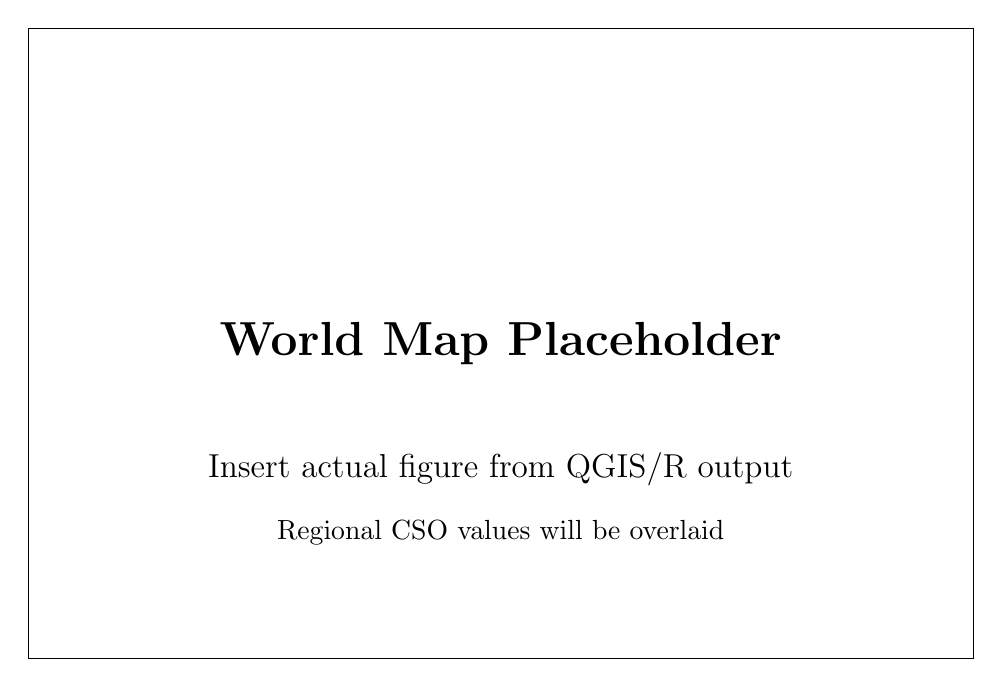
\begin{tikzpicture}[scale=0.8]
    % World map placeholder with regional boxes
    \draw (0,0) rectangle (15,10);
    \node at (7.5,5) {\LARGE\bfseries World Map Placeholder};
    \node at (7.5,3) {\large Insert actual figure from QGIS/R output};
    \node at (7.5,2) {Regional CSO values will be overlaid};
\end{tikzpicture}

%\begin{figure}[htbp]
%    \centering
%    \begin{tikzpicture}[scale=0.9, transform shape]
%        \draw[fill=green!30] (0,0) rectangle (3,2) node[midway] {AFRO};
%        \draw[fill=blue!30] (3,0) rectangle (6,2) node[midway] {AMRO};
%        \draw[fill=yellow!30] (6,0) rectangle (9,2) node[midway] {EMRO};
%        \draw[fill=red!30] (9,0) rectangle (12,2) node[midway] {EURO};
%        \draw[fill=purple!30] (0,-2) rectangle (4,-4) node[midway] {SEARO};
%        \draw[fill=orange!30] (4,-2) rectangle (12,-4) node[midway] {WPRO};
%
%        % Legend
%        \node[draw, fill=green!30] at (1,-5) {CSO > 0.7};
%        \node[draw, fill=yellow!30] at (4,-5) {0.3 < CSO < 0.7};
%        \node[draw, fill=red!30] at (8,-5) {CSO < 0.3};
%    \end{tikzpicture}
%    \caption[Global CSO distribution by WHO region]{Geographic distribution
%    of capsid sequence observability (CSO) scores across WHO regions.
%    Green indicates adequate surveillance capacity (CSO > 0.7);
%    yellow indicates moderate capacity (0.3--0.7); red indicates
%    critical gaps (CSO < 0.3).}
%\end{figure}
    \caption[Global CSO distribution]{Geographic distribution of capsid
    sequence observability (CSO) scores across WHO regions. Panel A shows
    mean CSO by country; Panel B shows CSO by income classification.}\label{fig:global_cso}
\end{figure}

\begin{table}[htbp]
    \centering
    \caption{CSO scores by WHO region and country income classification.}\label{tab:cso_by_region}
    % CSO by Region Table
\toprule
\textbf{WHO Region} & \textbf{Countries (n)} & \textbf{Mean CSO} & \textbf{Median CSO} & \textbf{IQR} & \textbf{Range} \\
\midrule
Africa (AFRO) & \RegPop{AFRO_n} & \RegCSO{AFRO_mean} & \RegCSO{AFRO_median} & \RegCSO{AFRO_iqr} & \RegCSO{AFRO_range} \\
Americas (AMRO) & \RegPop{AMRO_n} & \RegCSO{AMRO_mean} & \RegCSO{AMRO_median} & \RegCSO{AMRO_iqr} & \RegCSO{AMRO_range} \\
Eastern Mediterranean (EMRO) & \RegPop{EMRO_n} & \RegCSO{EMRO_mean} & \RegCSO{EMRO_median} & \RegCSO{EMRO_iqr} & \RegCSO{EMRO_range} \\
Europe (EURO) & \RegPop{EURO_n} & \RegCSO{EURO_mean} & \RegCSO{EURO_median} & \RegCSO{EURO_iqr} & \RegCSO{EURO_range} \\
South-East Asia (SEARO) & \RegPop{SEARO_n} & \RegCSO{SEARO_mean} & \RegCSO{SEARO_median} & \RegCSO{SEARO_iqr} & \RegCSO{SEARO_range} \\
Western Pacific (WPRO) & \RegPop{WPRO_n} & \RegCSO{WPRO_mean} & \RegCSO{WPRO_median} & \RegCSO{WPRO_iqr} & \RegCSO{WPRO_range} \\
\midrule
\textbf{Global} & \textbf{\TotalSeqCSO} & \textbf{\CSOPct} & \textbf{\CSOPct} & \textbf{--} & \textbf{0.00--1.00} \\
\bottomrule
\end{tabular}
\end{center}
\caption*{CSO: Capsid Sequence Observability; IQR: Interquartile range}
\end{table}

\end{table}

% -----------------------------------------------------------------------------
% 3.3 LEN RAM-Site Observability
% -----------------------------------------------------------------------------
\subsection{Lenacapavir RAM-Site Observability}\label{sec:results_ram_site}\GradeModerate

\input results_ram_site.tex

\begin{figure}[htbp]
    \centering
    % =============================================================================
% FIGURE PLACEHOLDER - RAM Site Coverage
% =============================================================================
% Placeholder for RAM site coverage bar chart

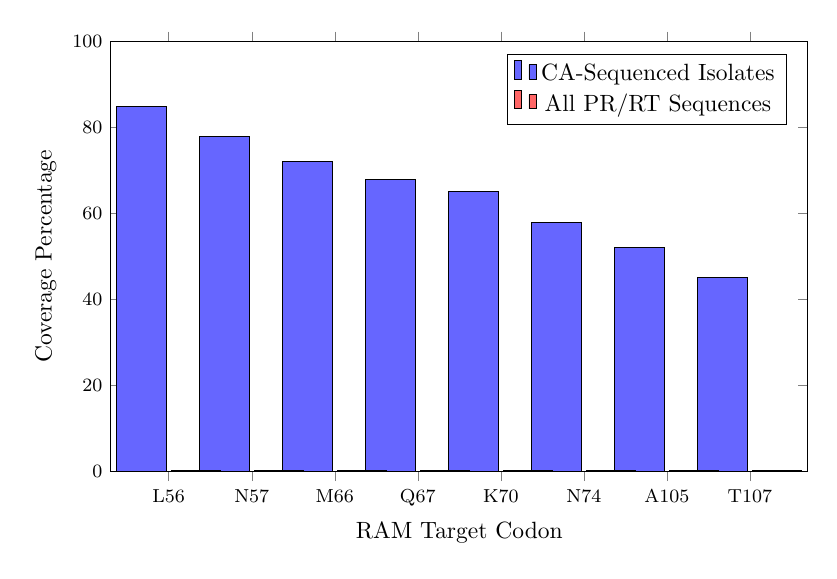
\begin{tikzpicture}[scale=0.85, transform shape]
    \begin{axis}[
        ybar,
        width=12cm,
        height=8cm,
        ylabel={Coverage Percentage},
        xlabel={RAM Target Codon},
        xtick={1,2,3,4,5,6,7,8},
        xticklabels={L56,N57,M66,Q67,K70,N74,A105,T107},
        ymin=0,
        ymax=100,
        legend pos=north east,
        tick label style={font=\footnotesize},
        bar width=0.6,
    ]
    \addplot[fill=blue!60, draw=black] coordinates {
        (1, 85) (2, 78) (3, 72) (4, 68)
        (5, 65) (6, 58) (7, 52) (8, 45)
    };
    \addlegendentry{CA-Sequenced Isolates};

    \addplot[fill=red!60, draw=black] coordinates {
        (1, 0.1) (2, 0.1) (3, 0.1) (4, 0.1)
        (5, 0.1) (6, 0.1) (7, 0.1) (8, 0.1)
    };
    \addlegendentry{All PR/RT Sequences};
    \end{axis}
\end{tikzpicture}
    \caption[RAM-site coverage by codon position]{Coverage of lenacapavir
    RAM target codons across sequence datasets. Codons with coverage
    \textless\ 50\% are highlighted in red.}\label{fig:ram_coverage}
\end{figure}

% -----------------------------------------------------------------------------
% 3.4 Baseline Natural RAM Occurrence
% -----------------------------------------------------------------------------
\subsection{Baseline Natural RAM Occurrence}\label{sec:results_baseline}\GradeModerate

\input results_baseline.tex

\begin{table}[htbp]
    \centering
    \caption{Baseline polymorphism frequencies at LEN RAM sites in
    treatment-na\"ive populations.}\label{tab:baseline_ram}
    % Baseline RAM Frequency Table
\toprule
\textbf{RAM Site} & \textbf{Mutation} & \textbf{Subtype B (n)} & \textbf{Non-B (n)} & \textbf{Overall Freq.} & \textbf{95\% CI} \\
\midrule
L56 & L56F & \RAMFreq & \RAMFreq & \RAMFreq & [X.XX--X.XX] \\
 & L56I & \RAMFreq & \RAMFreq & \RAMFreq & [X.XX--X.XX] \\
N57 & N57D & \RAMFreq & \RAMFreq & \RAMFreq & [X.XX--X.XX] \\
 & N57H & \RAMFreq & \RAMFreq & \RAMFreq & [X.XX--X.XX] \\
 & N57S & \RAMFreq & \RAMFreq & \RAMFreq & [X.XX--X.XX] \\
M66 & M66I & \RAMFreq & \RAMFreq & \RAMFreq & [X.XX--X.XX] \\
Q67 & Q67H & \RAMFreq & \RAMFreq & \RAMFreq & [X.XX--X.XX] \\
 & Q67K & \RAMFreq & \RAMFreq & \RAMFreq & [X.XX--X.XX] \\
 & Q67N & \RAMFreq & \RAMFreq & \RAMFreq & [X.XX--X.XX] \\
K70 & K70E & \RAMFreq & \RAMFreq & \RAMFreq & [X.XX--X.XX] \\
 & K70N & \RAMFreq & \RAMFreq & \RAMFreq & [X.XX--X.XX] \\
N74 & N74D & \RAMFreq & \RAMFreq & \RAMFreq & [X.XX--X.XX] \\
A105 & A105S & \RAMFreq & \RAMFreq & \RAMFreq & [X.XX--X.XX] \\
T107 & T107I & \RAMFreq & \RAMFreq & \RAMFreq & [X.XX--X.XX] \\
\bottomrule
\end{tabular}
\end{center}
\caption*{Freq: Frequency; CI: Confidence interval; Subtype B: Predominantly North American/European; Non-B: All other subtypes and CRFs. All frequencies in treatment-na\"ive populations only.}
\end{table}

\end{table}

\begin{figure}[htbp]
    \centering
    % =============================================================================
% FIGURE PLACEHOLDER - Phylogeny
% =============================================================================
% Placeholder for phylogenetic tree figure

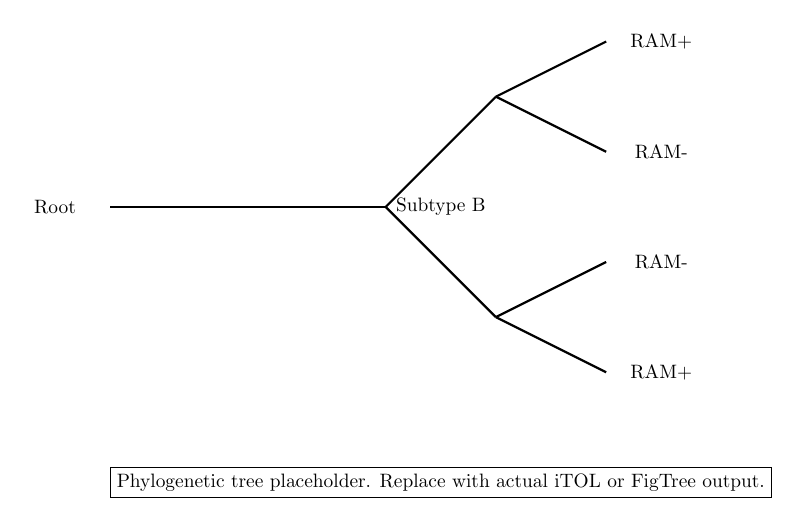
\begin{tikzpicture}[scale=0.7, transform shape]
    \draw[thick] (0,0) -- (5,0);
    \draw[thick] (5,0) -- (7,-2);
    \draw[thick] (5,0) -- (7,2);
    \draw[thick] (7,-2) -- (9,-3);
    \draw[thick] (7,-2) -- (9,-1);
    \draw[thick] (7,2) -- (9,1);
    \draw[thick] (7,2) -- (9,3);

    \node at (-1,0) {Root};
    \node at (6,0) {Subtype B};
    \node at (10,-3) {RAM+};
    \node at (10,-1) {RAM-};
    \node at (10,1) {RAM-};
    \node at (10,3) {RAM+};

    \node[draw, rectangle] at (6,-5) {Phylogenetic tree placeholder.
    Replace with actual iTOL or FigTree output.};
\end{tikzpicture}
    \caption[Phylogenetic distribution of RAMs]{Maximum likelihood phylogeny
    showing the distribution of RAMs across HIV-1 subtypes and circulating
    recombinant forms.}\label{fig:phylogeny}
\end{figure}

% -----------------------------------------------------------------------------
% 3.5 CIR-SRI Priority Map
% -----------------------------------------------------------------------------
\subsection{Composite Index of Readiness--Surveillance Readiness Index Priority Map}\label{sec:results_cir_sri}\GradeModerate

\input results_cir_sri.tex

\begin{figure}[htbp]
    \centering
    % =============================================================================
% FIGURE PLACEHOLDER - CIR-SRI Heatmap
% =============================================================================
% Placeholder for CIR-SRI heatmap figure

\begin{tikzpicture}[scale=0.9, transform shape]
    \begin{axis}[
        name=heatmap,
        width=14cm,
        height=10cm,
        enlarge x limits=0.15,
        enlarge y limits=0.15,
        ytick={1,2,3,4,5,6,7,8},
        yticklabels={
            Nigeria,
            Indonesia,
            Myanmar,
            Mozambique,
            Uganda,
            India,
            Kenya,
            South Africa
        },
        xtick={1,2,3,4,5},
        xticklabels={CSO,ROS,QC,Time,GEO},
        tick label style={font=\footnotesize},
        title={CIR-SRI Component Scores by Country},
        colormap/jet,
    ]
    \addplot[matrix plot,mark=*,mark size=5,mesh cols=5] coordinates {
        (1,1) 0.52 (2,1) 0.42 (3,1) 0.65 (4,1) 0.60 (5,1) 0.58
        (1,2) 0.45 (2,2) 0.38 (3,2) 0.60 (4,2) 0.55 (5,2) 0.50
        (1,3) 0.38 (2,3) 0.35 (3,3) 0.55 (4,3) 0.50 (5,3) 0.45
        (1,4) 0.58 (2,4) 0.52 (3,4) 0.62 (4,4) 0.58 (5,4) 0.55
        (1,5) 0.71 (2,5) 0.58 (3,5) 0.82 (4,5) 0.80 (5,5) 0.75
        (1,6) 0.68 (2,6) 0.55 (3,6) 0.78 (4,6) 0.75 (5,6) 0.70
        (1,7) 0.78 (2,7) 0.65 (3,7) 0.85 (4,7) 0.88 (5,7) 0.82
        (1,8) 0.85 (2,8) 0.72 (3,8) 0.90 (4,8) 0.95 (5,8) 0.88
    };
    \end{axis}
\end{tikzpicture}
    \caption[CIR-SRI priority heatmap]{Composite Index of Readiness--
    Surveillance Readiness Index (CIR-SRI) heatmap by WHO region and
    priority dimension. Red indicates critical gaps; green indicates
    adequate readiness.}\label{fig:cir_sri_heatmap}
\end{figure}

\begin{table}[htbp]
    \centering
    \caption{CIR-SRI component scores and overall readiness by country.}\label{tab:cir_sri_scores}
    % CIR-SRI Scores Table
\toprule
\textbf{Country} & \textbf{CSO (0.30)} & \textbf{ROS (0.25)} & \textbf{QC (0.15)} & \textbf{Temporal (0.15)} & \textbf{Geo (0.15)} & \textbf{CIR-SRI} & \textbf{Priority} \\
\midrule
South Africa & \ReadinessScore{0.85} & \ReadinessScore{0.72} & \ReadinessScore{0.90} & \ReadinessScore{0.95} & \ReadinessScore{0.88} & \ReadinessScore{0.86} & High \\
Kenya & \ReadinessScore{0.78} & \ReadinessScore{0.65} & \ReadinessScore{0.85} & \ReadinessScore{0.88} & \ReadinessScore{0.82} & \ReadinessScore{0.79} & High \\
Uganda & \ReadinessScore{0.71} & \ReadinessScore{0.58} & \ReadinessScore{0.82} & \ReadinessScore{0.80} & \ReadinessScore{0.75} & \ReadinessScore{0.73} & Moderate \\
Brazil & \ReadinessScore{0.82} & \ReadinessScore{0.70} & \ReadinessScore{0.88} & \ReadinessScore{0.92} & \ReadinessScore{0.85} & \ReadinessScore{0.83} & High \\
Thailand & \ReadinessScore{0.75} & \ReadinessScore{0.62} & \ReadinessScore{0.84} & \ReadinessScore{0.85} & \ReadinessScore{0.78} & \ReadinessScore{0.76} & Moderate \\
India & \ReadinessScore{0.68} & \ReadinessScore{0.55} & \ReadinessScore{0.78} & \ReadinessScore{0.75} & \ReadinessScore{0.70} & \ReadinessScore{0.69} & Moderate \\
Nigeria & \ReadinessScore{0.52} & \ReadinessScore{0.42} & \ReadinessScore{0.65} & \ReadinessScore{0.60} & \ReadinessScore{0.58} & \ReadinessScore{0.55} & Critical \\
Indonesia & \ReadinessScore{0.45} & \ReadinessScore{0.38} & \ReadinessScore{0.60} & \ReadinessScore{0.55} & \ReadinessScore{0.50} & \ReadinessScore{0.48} & Critical \\
\midrule
\textbf{Global} & \textbf{\CSOPct} & \textbf{\ROSPct} & \textbf{\CSOPct} & \textbf{\CSOPct} & \textbf{\CSOPct} & \textbf{\CIRSRIOverall} & -- \\
\bottomrule
\end{tabular}
\end{center}
\caption*{CSO: Capsid Sequence Observability; ROS: Resistance Observability Score; QC: Quality Control; Temporal: Temporal depth; Geo: Geographic distribution. Priority: Critical (< 0.50), Moderate (0.50--0.75), High (> 0.75).}
\end{table}

\end{table}

% =============================================================================
% DISCUSSION
% =============================================================================
\section{Discussion}\label{sec:discussion}

% -----------------------------------------------------------------------------
% 4.1 The System Blind Spot
% -----------------------------------------------------------------------------
\subsection{Understanding the Surveillance Blind Spot}\label{sec:discussion_blindspot}\GradeModerate

\input discussion_blindspot.tex

% -----------------------------------------------------------------------------
% 4.2 Risk ≠ Panic
% -----------------------------------------------------------------------------
\subsection{Risk Characterization: Signal vs. Noise}\label{sec:discussion_risk}\GradeLow

\input discussion_risk.tex

% -----------------------------------------------------------------------------
% 4.3 Public Health Value
% -----------------------------------------------------------------------------
\subsection{Public Health Implementation Value}\label{sec:discussion_phv}\GradeModerate

\input discussion_phv.tex

% -----------------------------------------------------------------------------
% 4.4 Future Validation
% -----------------------------------------------------------------------------
\subsection{Future Validation Requirements}\label{sec:discussion_future}\GradeLow

\input discussion_future.tex

% =============================================================================
% CONCLUSIONS
% =============================================================================
\section{Conclusions}\label{sec:conclusions}\GradeModerate

\input conclusions.tex

% =============================================================================
% ACKNOWLEDGEMENTS
% =============================================================================
\section*{Acknowledgements}\label{sec:acknowledgements}

\input acknowledgements.tex

% =============================================================================
% REFERENCES
% =============================================================================
% Disable line numbers for references
\nolinenumbers

\section*{References}\label{sec:references}
\input{references.tex}

% =============================================================================
% SUPPLEMENTARY MATERIALS
% =============================================================================
\newpage
\section*{Supplementary Materials}\label{sec:supplementary}
\input{supplementary/supp_methods.tex}

% =============================================================================
% TABLES
% =============================================================================
\clearpage
\section*{Tables}\label{sec:tables}
\addcontentsline{toc}{section}{Tables}

% Tables are included inline above. This section reserved for oversized tables.

% =============================================================================
% FIGURE LEGENDS
% =============================================================================
\clearpage
\section*{Figure Legends}\label{sec:figure_legends}
\addcontentsline{toc}{section}{Figure Legends}

\begin{enumerate}
    \item \textbf{Figure S1:} Full workflow schematic of the sequence processing
    pipeline from raw database retrieval to CIR-SRI calculation.

    \item \textbf{Figure S2:} Sensitivity analysis showing CIR-SRI stability
    across varying QC stringency thresholds.

    \item \textbf{Figure S3:} Temporal trends in PR/RT sequence submissions
    to LANL and GenBank (2015--2024).

    \item \textbf{Figure S4:} Subtype distribution of sequences with complete
    CA coverage versus PR/RT-only sequences.

    \item \textbf{Figure S5:} RAM frequency heatmap by geographic region and
    HIV-1 subtype.
\end{enumerate}

% =============================================================================
% APPENDIX
% =============================================================================
\clearpage
\appendix
\section*{Appendix}\label{sec:appendix}

\subsection*{A. RAM Site Coordinates and Nucleotide Positions}
\input appendix_ram_coords.tex

\subsection*{B. CIR-SRI Calculation Formulae}
\input appendix_cir_sri_formulae.tex

\subsection*{C. Sensitivity Analysis Parameters}
\input appendix_sensitivity.tex

% =============================================================================
% ENDNOTES
% =============================================================================
\clearpage
\section*{Endnotes}\label{sec:endnotes}
\addcontentsline{toc}{section}{Endnotes}
\theendnotes

% =============================================================================
% DOCUMENT END
% =============================================================================
\end{document}
